\documentclass[UROP.tex]{subfiles}
\begin{document}

\bigskip
\section{\Large Background}
	Phased array systems have been designed before for different use cases, and at different frequencies.  A phased array allows for fast steering of a very directed beam.  Higher frequency phased arrays have been used for this application, however these phased arrays have limited range because of the high attenuation constants at high frequencies.  This phased array system shall work at distances up to 20 miles.  All previous phased arrays designed for this purpose are on a single plane; we are designing a 3D array to obtain higher gain at lower elevation angles. \\
	
	Members in our group are well educated in antenna design: some members have worked in RF research labs, and others at RF companies.  
	
\begin{figure}[H]
\centering
	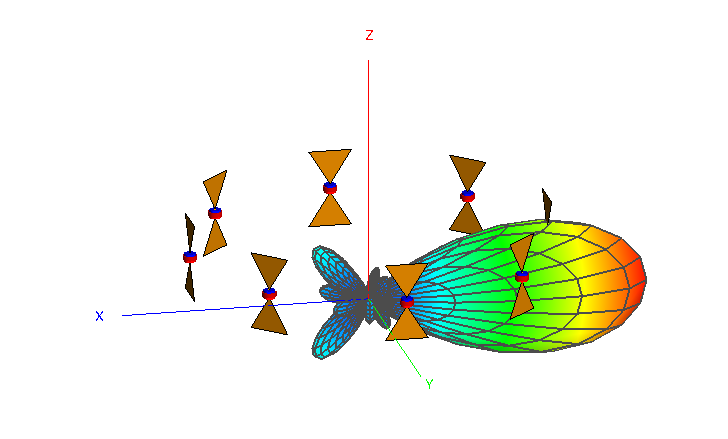
\includegraphics[scale=0.4]{PhasedArrayExample.png}
	\caption{ Phased Array example showing the ability to steer a beam\label{fig:PAexample}}
\end{figure}
	
	As seen in Fig.~\ref{fig:PAexample}, the ability to steer a beam is inherent in the design of a phased array.  This array is a preliminary design to the 3D array that will be the final product.  Some of the students in this group worked with phased array systems, and will use that experience to design a better, longer range phased array system.  
\end{document}
